
%=========================================================
\chapter{Planeación de Capital Humano}	
\label{cap:capHumano}

	En este capítulo se presenta la planeación del capital humano del proyecto. Se especifican los integrantes, el organigrama, las habilidades de cada integrante, así como sus roles y responsabilidades en el proyecto.

%---------------------------------------------------------
\section{Organigrama}	

\cdtInstrucciones{
	Arme un diagrama jerárquico que capture la cadena de mando o de  información en el proyecto identificando los principales roles en el equipo de trabajo del proyecto.
}

En la figura~\ref{fig:organigrama} se presentan los roles y la cadena de mando en el proyecto. 

\begin{figure}[htbp]
	\begin{center}
		\fbox{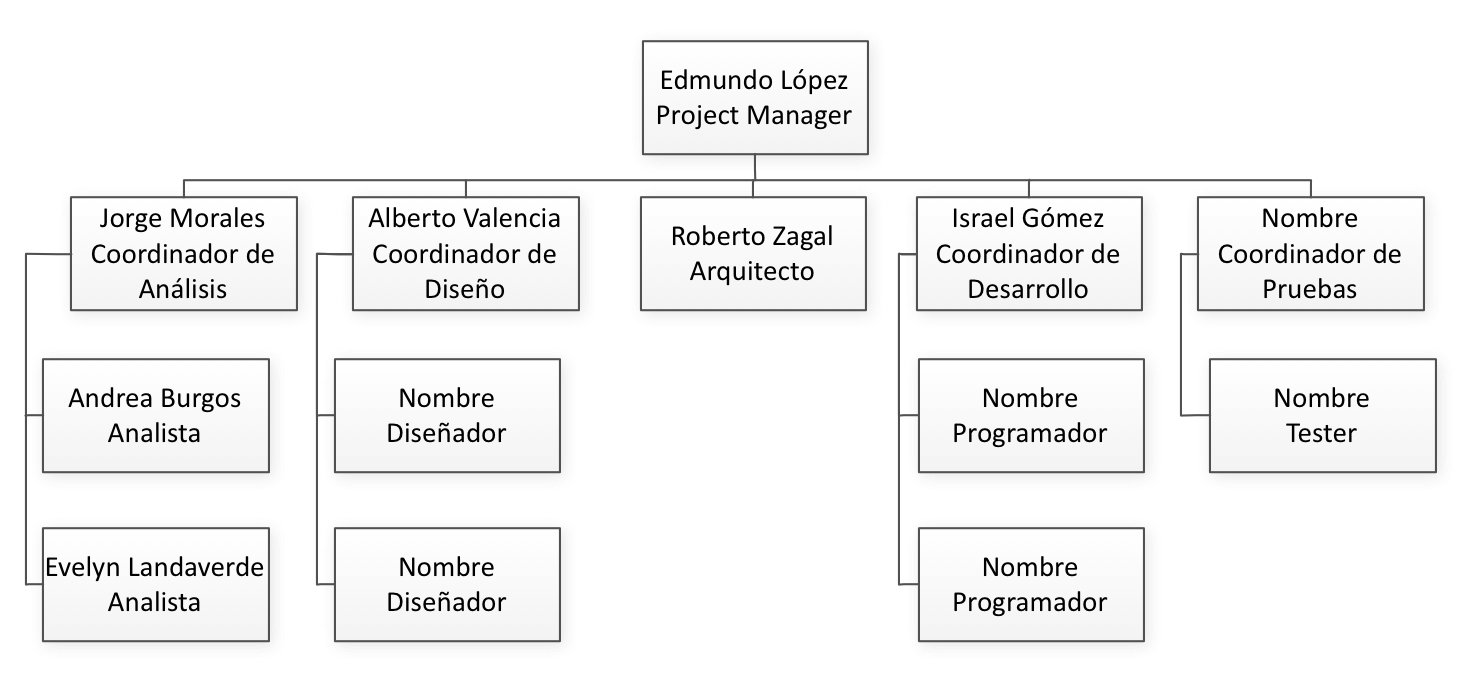
\includegraphics[width=.8\textwidth]{images/organigrama}}
		\caption{Organigrama del proyecto}
		\label{fig:organigrama}
	\end{center}
\end{figure}


%---------------------------------------------------------
\section{Responsabilidades}

\cdtInstrucciones{
	Para cada Rol en el proyecto especifique una descripción, responsabilidades dentro del proyecto y habilidades o perfil que se debe cubrir para el puesto.
}


\subsection{Project Manager}
	Líder de proyecto y encargado de el cumplimiento del objetivo del proyecto.

\begin{description}
	\item[Responsabilidades:] \cdtEmpty 	
    \begin{itemize}
    	\item Reconocer los riesgos que puedan impactar la probabilidad de éxito del proyecto.
		\item Crear políticas para reducir el impacto de los riesgos.
		\item ...
    \end{itemize}
	\item[Perfil:] \cdtEmpty	
    \begin{itemize}
       	\item Licenciado en ...
		\item Conocimientos básicos de tecnologías de información y uso de internet.
		\item Experiencia liderando proyectos.
		\item ...
    \end{itemize}
\end{description}

%---------------------------------------------------------
\section{Staff}

\cdtInstrucciones{
	Liste a los integrantes del proyecto especificando su rol, y datos de contacto.\\
}

\begin{table}[hbtp!]
    \noindent\begin{tabular}{|p{.25\textwidth}|p{.15\textwidth}|p{.12\textwidth}|p{.15\textwidth}|p{.15\textwidth}|}
    	\hline
    	{\bf Nombre} & {\bf Rol} & {\bf Horario} & {\bf Teléfonos} & {\bf Correo}\\
    	\hline
    	Juan Crisóstomo & Programador & 4:00 -- 16:00 & 5576-6777 & juan@ipn.mx \\
    	\hline
    	... & ... & ... & ... & ... \\
    	\hline
    \end{tabular}
	\caption{Integrantes del proyecto.}
	\label{tbl:staff}
\end{table}

